\section{Penelitian Terkait}
\label{sec:penelitian-terkait}
Beberapa pendahulu penulis di Departemen Teknik Transportasi Laut Fakultas Teknologi Kelautan ITS telah menghasilkan sejumlah tugas akhir yang bertujuan untuk meningkatkan efisiensi dan efektivitas distribusi bahan bakar minyak (BBM) melalui transportasi laut di wilayah Indonesia. Tugas-tugas akhir tersebut mengangkat distribusi BBM sebagai fokus penelitian yang mendalam. Melalui penelitian-penelitian sebelumnya, berbagai aspek terkait dengan distribusi BBM telah diteliti dengan tujuan untuk mengidentifikasi solusi-solusi inovatif dalam mengatasi tantangan distribusi BBM di wilayah Indonesia.
    
    Penelitian oleh Nabila Hidni \citep{Hidni2016Model} menyoroti tantangan dalam mempertahankan pasokan BBM yang memadai di wilayah tujuan ketika armada kapal tanker inti sedang tidak tersedia. Kendala ini memicu permasalahan dalam keamanan pasokan, terutama di wilayah Indonesia Timur, karena sulitnya mencari kapal pengganti dengan harga sewa yang terjangkau dan dalam waktu yang singkat. Irfa'atil Karimah \citep{Karimah2016Optimalisasi} menjelaskan upaya optimalisasi kepemilikan armada tanker untuk memastikan distribusi BBM yang paling ekonomis, dengan mengidentifikasi model kepemilikan dan pola operasi yang paling efisien.

    Selanjutnya, penelitian oleh Ni Putu Intan Pratiwi \citep{Pratiwi2013Internalisasi} menekankan pentingnya internalisasi biaya eksternal dalam perhitungan unit cost pengangkutan BBM. Penelitian ini mencoba memodelkan dampak jika biaya-biaya eksternal seperti demurrage, biaya polusi, dan biaya kongesti dimasukkan secara langsung dalam perhitungan biaya transportasi laut. Internalisasi biaya-biaya ini diharapkan dapat memberikan gambaran yang lebih akurat tentang biaya sebenarnya dalam distribusi BBM dan mendorong pemangku kepentingan untuk mencari solusi yang lebih efisien dan berkelanjutan.
    
    Terakhir, penelitian oleh Putra Alhamda \citep{Alhamda2016Optimalisasi} menggali alternatif distribusi BBM di wilayah kepulauan, dengan fokus pada Nusa Tenggara Barat (NTB). Studi ini membandingkan biaya logistik BBM antara penggunaan kapal tanker dan kapal petikemas, serta pembangunan kapal petikemas baru. Hasilnya menunjukkan bahwa penggunaan kapal petikemas dapat menjadi pilihan yang lebih ekonomis dengan syarat infrastruktur pelabuhan mendukung, menunjukkan peran pentingnya infrastruktur dalam menentukan efisiensi sistem distribusi BBM.



\begin{comment}
Dinamika sistem atau \emph{System Dynamic} pertama kali dikembangkan oleh Jay Forrester, seorang profesor dari MIT pada pertengahan tahun 1950. Ide dasar yang mengawali dinamika sistem adalah penerapan hukum-hukum fisika khususnya sirkuit elektronik dalam dinamika ekonomi dan dilanjutkan di bidang sosial. Dasar-dasar dan bahasa pemodelan disusun pada akhir tahun 1950 hingga 1960 dan tidak berubah hingga sekarang \citep{stermanBusinessDynamicsSystems2009}.
Konsep utama simulasi dinamika sistem adalah interaksi antar elemen dan perubahan nilai suatu elemen dari waktu ke waktu. Konsep tadi diwujudkan dengan bentuk \emph{stock} untuk memodelkan suatu elemen dan \emph{flow} untuk memodelkan interaksi antar elemennya.

Dinamika sistem sudah digunakan untuk meneliti masalah sosial ekonomi dan proyeksi emisi, sebagaimana yang dilakukan Liu dkk. (2019) yang memodelkan emisi yang dihasilkan pada hinterland pelabuhan dengan interaksi antara waktu transportasi, armada truk yang digunakan dan volume muatan yang dibawa \citep{liuSystemDynamicsModel2019}.

\begin{figure}[ht]
  \centering
  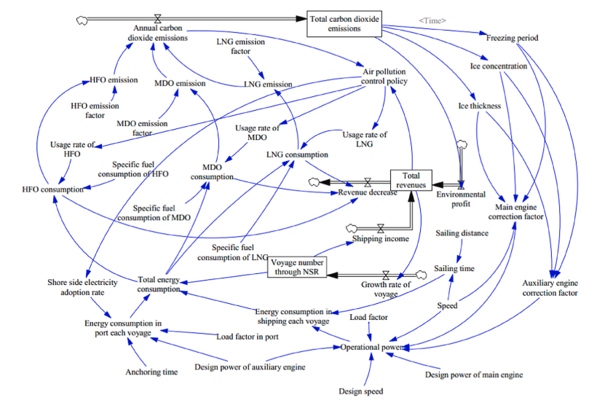
\includegraphics[scale=0.75]{gambar/gambar-dinamika-sistem-LB.png}
  \caption{Model dinamika sistem untuk memproyeksikan emisi pelayaran arktik dan interaksinya dengan unsur-unsur pelayaran menurut \citet{jingCO2EmissionProjection2021}.}
  \label{fig:contoh-model-dinamika-sistem}
\end{figure}

Penelitian yang dilakukan Huang dkk. (2017) menggunakan dinamika sistem untuk memodelkan emisi dari kapal dalam wilayah Pelabuhan Tianjin. Model dibuat untuk mengetahui hubungan antara keuntungan yang diperoleh pelabuhan dan emisi yang dihasilkan di kawasan pelabuhan dengan memerhatikan faktor kebijakan ekonomi dan unsur-unsur teknik di pelabuhan \citep{huangSystemDynamicsModeling2017}.

Selain dinamika sistem terdapat metode simulasi diskrit dan simulasi berbasis agen. Perbedaan metode simulasi tersebut terletak pada seberapa detail skala model atau level abstraksi yang diinginkan. Pemilihan simulasi dinamika sistem dikarenakan level abstraksi sistem yang bersifat lebih luas dan menangkap kondisi secara makro. Interaksi antar variabel dan dampaknya terhadap hal utama yang ingin diteliti juga dapat diamati dengan simulasi dinamika sistem \citep{borshchevBigBookSimulation2013}.
\end{comment}